\chapter{Introducción Específica}
\label{Chapter2}

En el presente capítulo se brinda una explicación del funcionamiento general del sistema implementado, y una introducción a diferentes tecnologías utilizadas en el trabajo. Se presentan además los requerimientos y la planificación del trabajo.

\section{Funcionamiento general del sistema}
\label{funcionamiento_general}

Como se mencionó en el capítulo \ref{chapter1}, el propósito del presente trabajo es el desarrollo de un módulo capaz de dotar de conectividad WiFi/Bluetooth a un electrodoméstico convencional. Para que ello sea posible, es necesario contar con diferentes módulos, tal como puede observarse en la figura \ref{fig:simplified_diagram}, en la que se presenta un diagrama de bloques del sistema implementado. 

\begin{figure}[h]
\centering
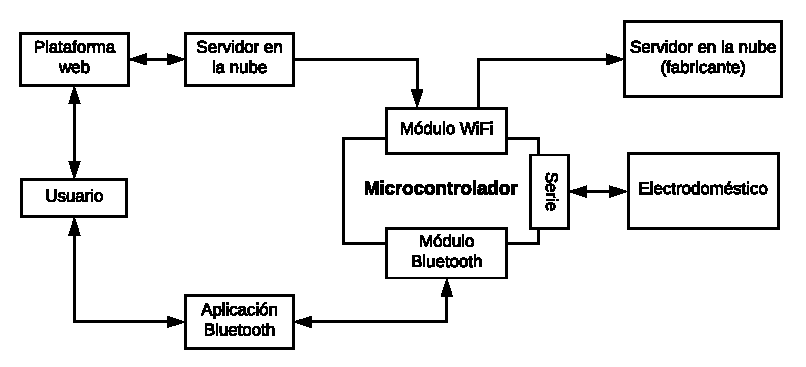
\includegraphics[width=\textwidth]{./Figures/simplified_diagram.pdf}
\caption{Diagrama general del sistema implementado.}
\label{fig:simplified_diagram}
\end{figure}

El principal componente del sistema es el microcontrolador, que se encarga de procesar los comandos recibidos y de gestionar todas las comunicaciones, para lo que hace uso de sus interfaces de comunicación (módulos WiFi, Bluetooth y serie).

Con el fin de ilustrar el funcionamiento general del sistema, se presenta a continuación la serie de acciones que tiene lugar en un caso de uso típico del sistema, en el que el usuario desea que el electrodoméstico inicie una determinada operación (como por ejemplo, el ciclo de lavado en un lavarropas).

\begin{itemize}
	\item El usuario final le envía un comando al electrodoméstico desde su computadora o celular.
	\begin{itemize}
		\item En caso de que el comando sea enviado por WiFi, la comunicación pasa a través de un servidor en la nube que recibe el comando del usuario y luego lo envía al microcontrolador.
		\item En caso de que el comando sea enviado por Bluetooth, la comunicación se realiza de manera directa con el microcontrolador.
	\end{itemize}
	\item El módulo correspondiente (WiFi o Bluetooth, según sea el caso) recibe el comando y le informa al microcontrolador que hay un nuevo comando pendiente para procesar.
	\item El microcontrolador procesa el comando recibido y determina la acción a ejecutar.
	\item Si la acción a ejecutar lo requiere, el microcontrolador se comunica con la placa de control del electrodoméstico mediante una interfaz serie, a los fines de disparar en el mismo la operación deseada por el usuario.
	\item Dependiendo del tipo de acción, el electrodoméstico puede contestar con su información de estado. Esta es recibida por el microcontrolador y enviada de vuelta al usuario a través de la misma interfaz desde la cual recibió el comando originalmente. Es decir que si el usuario envió un comando por Bluetooth para consultar el estado del artefacto, el microcontrolador utiliza el módulo Bluetooth para devolverle la respuesta.
\end{itemize}

Cabe mencionar que debido a limitaciones de hardware, las interfaces de comunicación WiFi y Bluetooth no pueden ser utilizadas en simultáneo. Por lo tanto, si se envían comandos por WiFi, el Bluetooth debe estar apagado, y viceversa al enviar comandos por Bluetooth. 

De manera independiente a las acciones disparadas a partir de un comando del usuario, el microcontrolador envía periódicamente al fabricante información acerca del estado del electrodoméstico. Este envío se lleva a cabo mediante la interfaz WiFi, que se comunica con un servidor en la nube solamente accesible por el fabricante, y que se encarga de almacenar la información para luego permitir su análisis y visualización. Gracias a esta información, el fabricante puede conocer y visualizar en todo momento el estado de sus electrodomésticos, ya sea de manera individual con todo el historial de uso de cada uno, o de forma general agrupando artefactos para obtener un panorama global del estado de sus dispositivos conectados.

Además, el módulo crea y mantiene activa en todo momento una red WiFi local de corto alcance en la que se encuentra corriendo un servidor web. El usuario puede conectarse a esta red y luego acceder desde cualquier navegador de Internet al servidor web, que permite configurar las credenciales de la red WiFi doméstica a la cual el módulo se conectará para recibir comandos y enviar información de uso al fabricante.

\section{Tecnologías inalámbricas}

En la actualidad, existen numerosas tecnologías inalámbricas que son aplicables a la Internet de las Cosas, muchas de las cuales surgieron debido a la relevancia que este concepto fue tomando, como es el caso de NB-IoT \citep{nb_iot}, LoRa \citep{lora} y SigFox \citep{sigfox}. Gran parte de estas tecnologías se caracterizan por permitir un bajo consumo de potencia y un largo alcance, a costa de una baja velocidad de transmisión. En muchas ocasiones esto es una relación de compromiso ideal para Internet de las Cosas.

A pesar del surgimiento de estas nuevas redes, las tecnologías tradicionales de conectividad inalámbrica, como el WiFi \citep{wifi} y el Bluetooth \citep{bluetooth}, siguen siendo adecuadas para muchas aplicaciones, especialmente aquellas que requieren una interacción directa con el usuario final. Esto se debe a que son tecnologías ampliamente soportadas por la mayoría de los dispositivos que posee una persona, como computadoras y celulares.

Un electrodoméstico conectado interactúa de manera directa con la persona que lo utiliza en el hogar, por lo tanto el WiFi y el Bluetooth son tecnologías sumamente adecuadas para un módulo destinado a tal fin.

La tecnología WiFi permite transmitir a grandes velocidades, pero con un alcance bajo y un consumo de energía mayor. Esto último impide que el WiFi sea utilizado en, por ejemplo, sensores que funcionan a batería ubicados en lugares remotos, pero no supone un problema para un electrodoméstico que se encuentra en el hogar, con fácil acceso a una fuente de alimentación y cerca de un punto de acceso al cual conectarse. 

Las especificaciones del WiFi definen una interfaz que se emplea para enviar y recibir señales entre un dispositivo inalámbrico (estación WiFi) y un punto de acceso. Si además se requiere tener acceso a Internet, es necesario conectarse también con un \emph{router} y un módem, que a su vez debe estar conectado a un proveedor de servicios de Internet (ISP, por sus siglas en inglés correspondientes a \emph{Internet Service Provider}). El módulo en el electrodoméstico actúa como una estación WiFi, es decir como un dispositivo que se conecta a la red doméstica de la casa y a través de ella obtiene una salida a Internet.

Por su parte, la tecnología Bluetooth pertenece a otro tipo de redes, denominadas Redes de Área Personal (PAN, por sus siglas en inglés). Una conexión Bluetooth permite la comunicación directa entre dos dispositivos cercanos y su uso está sumamente masificado, ya que es fácil y económico integrarlo en muchos aparatos. Estas son características que lo convierten en una tecnología ideal para utilizar en un electrodoméstico conectado.

Su utilización en el ámbito de la Internet de las Cosas cobró verdadera importancia gracias al surgimiento del Bluetooth Low Energy (BLE), que fue diseñado específicamente para proporcionar un bajo consumo de energía. Esto permitió incrementar aún más la popularidad de la tecnología, y extenderla hacia nuevos dispositivos como relojes o incluso zapatillas, lo cual fue acompañado con cada vez más modelos de computadores y celulares que también soporten la tecnología.


\section{Protocolos HTTP/S y MQTT}

Para que un dispositivo pueda conectarse a Internet, necesariamente debe recurrir al modelo TCP/IP \citep{tcp_ip_model}, cuyas diferentes capas pueden observarse en la figura \ref{fig:modelo_tcp_ip}.

\begin{figure}[h]
\centering
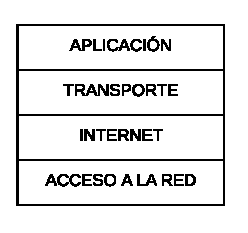
\includegraphics{./Figures/modelo_tcp_ip.pdf}
\caption{Capas del modelo TCP/IP.}
\label{fig:modelo_tcp_ip}
\end{figure}

El protocolo a nivel de capa de acceso a la red depende del hardware y del tipo de conectividad del dispositivo, y en el caso de este trabajo está constituido por la tecnología WiFi. Las capas de Internet y de transporte utilizan, en este trabajo, los protocolos que le dan el nombre al modelo, es decir IP (\emph{Internet Protocol}) y TCP (\emph{Transmission Control Protocol)}), respectivamente.

La capa de aplicación, ubicada en la parte superior del modelo, es la encargada de ofrecer a las aplicaciones de usuario la posibilidad de comunicarse con otros dispositivos a través de los servicios brindados por las demás capas.

El protocolo de aplicación más conocido es el Protocolo de Transferencia de Hipertexto (HTTP por sus siglas en inglés, correspondientes a \emph{Hypertext Transfer Protocol}), que tiene una estructura cliente-servidor y permite realizar peticiones de datos y recursos \citep{http_protocol}. Este protocolo es la base de cualquier intercambio de datos en la web, y por lo tanto es utilizado en aplicaciones de Internet de las Cosas cuando se desea que el dispositivo conectado acceda directamente a diferentes páginas web.

Existe una variante denominada Protocolo Seguro de Transferencia de Hipertexto (HTTPS por sus siglas en inglés, correspondientes a \emph{Hypertext Transfer Protocol Secure}), que como su nombre lo indica, es una versión segura de HTTP en la que la transmisión está encriptada y el servidor, autenticado \citep{https_protocol}. En toda aplicación, siempre se debe hacer lo posible para utilizar HTTPS y no simplemente HTTP, con el fin de garantizar la seguridad y la privacidad de los datos.

Además de los protocolos HTTP y HTTPS, existen otros para la capa de aplicación con características que los hacen ideales para la Internet de las Cosas, entre los que se destaca el protocolo MQTT (\emph{Message Queue Telemetry Transport}) \citep{mqtt_protocol}. Este protocolo se basa en un modelo de publicaciones y subscripciones, en el que un cliente publica mensajes en un tema o \emph{topic}, y todos aquellos nodos que se encuentran subscriptos a ese tema reciben el mensaje publicado. MQTT es ideal para aplicaciones de IoT, debido principalmente a que requiere un muy bajo ancho de banda, tiene un menor consumo de potencia que otras alternativas, y además es sencillo y ligero de implementar.

Por todo lo enunciado anteriormente es que se decide que el módulo desarrollado soporte los 3 protocolos: HTTP, HTTPS y MQTT.

\section{Requerimientos}
\label{requerimientos}

A continuación se presentan los requerimientos en base a los cuales se desarrolló el presente trabajo, agrupados en cuatro categorías.
\begin{enumerate}
	\item Requerimientos generales del sistema.
	\begin{enumerate}
		\item El módulo debe ser capaz de llevar a cabo, mediante la recepción de comandos por
WiFi o Bluetooth, las mismas funciones que a través de la interfaz física del
electrodoméstico.
		\item El módulo debe ser capaz de enviar comandos por WiFi o Bluetooth, para transmitir información de estado del electrodoméstico.
		\item Las acciones a ejecutar de acuerdo al comando recibido dependen de cada
aparato en particular, pero como mínimo se debe brindar la posibilidad de iniciar o
detener la acción del electrodoméstico y consultar su estado.
		\item El módulo debe enviar al fabricante información asociada al uso del
electrodoméstico, e informar periódicamente el estado en el que se encuentra.
		\item El módulo debe ser capaz de crear su propia red local WiFi a los fines de permitir configurar las credenciales de de la red WiFi a conectarse.
		\item El módulo debe ser capaz de enviar y recibir comandos por WiFi utilizando los
protocolos HTTP, HTTPS y MQTT.
	\end{enumerate}
	\item Requerimientos de hardware.
	\begin{enumerate}
		\item El módulo debe poder comunicarse utilizando el Estándar IEEE 802.11 b/g/n
(WiFi).
		\item El módulo debe poder comunicarse utilizando Bluetooth Low Energy (BLE).
		\item El módulo debe utilizar un único chip que integre el microprocesador y la conectividad WiFi/Bluetooth.
		\item El módulo debe contar como mínimo con interfaces de comunicación serie SPI (\emph{Serial Peripheral Interface}), I2C (\emph{Inter-Integrated Circuit}) y UART (\emph{Universal Asynchronous Receiver-Transmitter}), a los fines de poder adaptarse a los distintos tipos de electrodomésticos.
	\end{enumerate}
	\item Requerimientos de firmware.
	\begin{enumerate}
		\item El firmware del módulo debe ser programado en lenguaje C.
		\item Se deben realizar pruebas manuales para cada una de las funcionalidades del firmware del módulo.
	\end{enumerate}
	\item Requerimientos de gestión de proyectos.
	\begin{enumerate}
		\item Se debe utilizar YouTrack \citep{youtrack} como herramienta de \emph{issue tracking} y gestión de proyectos.
		\item Se debe usar Git como sistema de control de versiones.
	\end{enumerate}
\end{enumerate}

Cabe mencionar en este punto que originalmente se había planteado la integración del módulo a un electrodoméstico real, lo que implicaba también el diseño y fabricación de un PCB que se adaptase a él. Sin embargo, debido a las dificultades para acceder a un electrodoméstico sobre el cual probar el módulo, sumado a la necesidad de acelerar los tiempos de desarrollo, se decidió reemplazar dicho electrodoméstico por otro microcontrolador que emulase su comportamiento.


\section{Planificación}

Para mostrar la planificación del trabajo se recurre a un diagrama \emph{Activity On Node} (figuras \ref{fig:activity_on_node_1}, \ref{fig:activity_on_node_2} y \ref{fig:activity_on_node_3}). Allí cada caja o nodo representa una actividad, y las conexiones entre ellas representan una dependencia temporal en la que una debe terminarse antes que la siguiente. Además se muestra el tiempo en horas que demoraría cada una de las tareas. En la tabla \ref{tab:codigo_colores} se explica el significado de cada color del diagrama.

\begin{table}[h]
	\centering
	\caption{Código de colores del diagrama Activity On Node.}
	\begin{tabular}{l l}    
		\toprule
		\textbf{Color}	& \textbf{Significado}				\\
		\midrule
		Violeta			& Planificación						\\
		Gris			& Análisis e investigación			\\
		Rosa			& Ingeniería de software			\\
		Naranja			& Hardware							\\
		Rojo			& Desarrollo de firmware			\\
		Verde claro		& Pruebas							\\
		Celeste 		& Interfaz							\\
		Verde oscuro 	& Presentación						\\
		\bottomrule
		\hline
	\end{tabular}
	\label{tab:codigo_colores}
\end{table}

\begin{figure}[h]
\centering
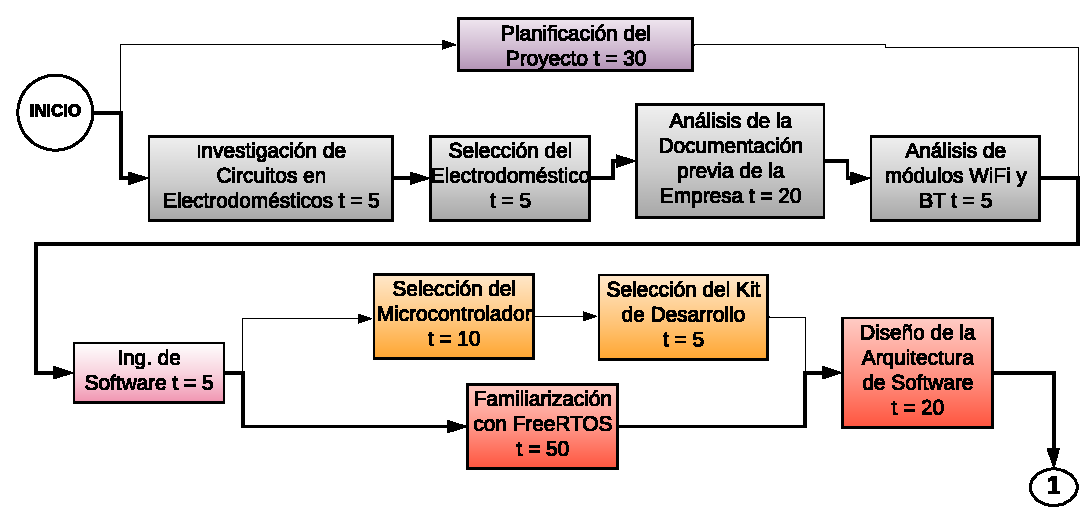
\includegraphics[width=\textwidth]{./Figures/activity_on_node_1.pdf}
\caption{Diagrama Activity On Node parte 1.}
\label{fig:activity_on_node_1}
\end{figure}

Se puede observar que la primera etapa consiste en análisis e investigación, además de la planificación del trabajo. Luego sigue una etapa de diseño de firmware y familiarización con las herramientas a utilizar, sin empezar aún con la implementación.

\begin{figure}[h]
\centering
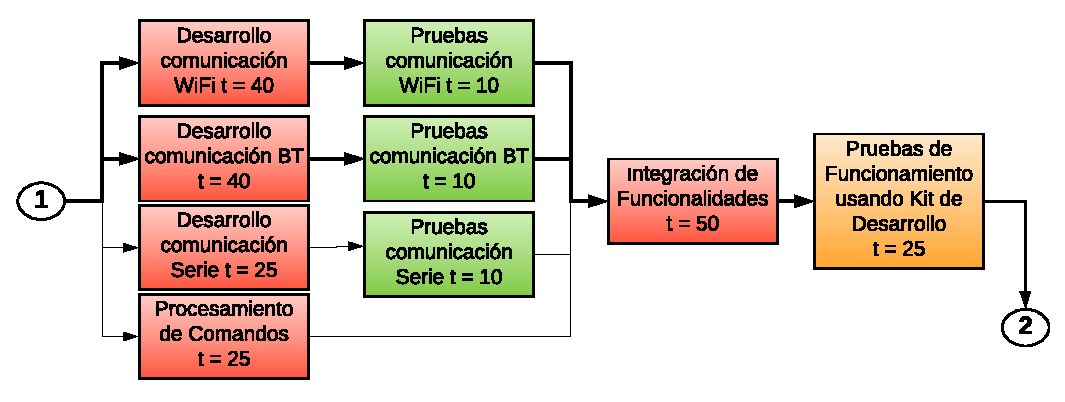
\includegraphics[width=\textwidth]{./Figures/activity_on_node_2.pdf}
\caption{Diagrama Activity On Node parte 2.}
\label{fig:activity_on_node_2}
\end{figure}

Una vez definido el diseño, se procede con el desarrollo de las diferentes funcionalidades de firmware y sus respectivas pruebas. Si bien en el diagrama (figura \ref{fig:activity_on_node_2}) la realización de estas tareas se muestra en paralelo, ya que son relativamente independientes y por lo tanto podrían ejecutarse en simultáneo, al ser desarrollado por una única persona, las tareas se debieron desarrollar en serie.

Luego se integran todas las funcionalidades implementadas y se realizan pruebas generales del sistema, para posteriormente configurar las plataformas utilizadas para enviar y recibir información por WiFi y Bluetooth.

\begin{figure}[h]
\centering
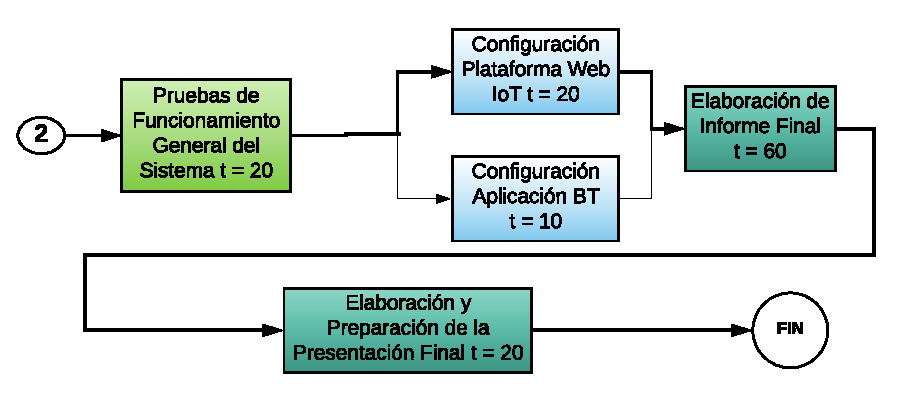
\includegraphics[width=\textwidth]{./Figures/activity_on_node_3.pdf}
\caption{Diagrama Activity On Node parte 3.}
\label{fig:activity_on_node_3}
\end{figure}

Por último se contempla también el tiempo necesario para las actividades asociadas a la presentación del trabajo final.

%
%\begin{figure}[h]
%\centering
%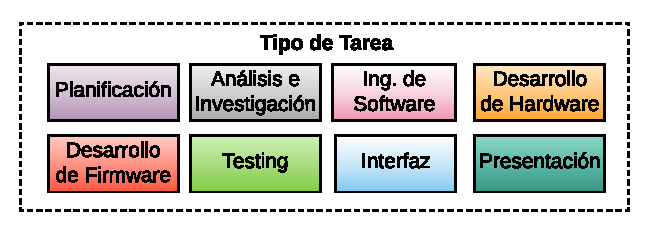
\includegraphics[width=\textwidth]{./Figures/activity_on_node_4.pdf}
%\caption{Referencias del diagrama Activity On Node.}
%\label{fig:activity_on_node_4}
%\end{figure}


